\documentclass[onecolumn, draftclsnofoot,10pt, compsoc]{IEEEtran}

\usepackage{graphicx}
\usepackage{url}
\usepackage{setspace}
\usepackage{geometry}
\usepackage{listings}
\usepackage{xcolor}

\lstset{basicstyle=\ttfamily,
  showstringspaces=false,
  commentstyle=\color{red},
  keywordstyle=\color{blue}
}

\graphicspath{ {./images/} }
\geometry{margin = 0.75in}

% ---- Removes "References" from bibliography section ----
\usepackage{etoolbox}
\patchcmd{\thebibliography}{\section*{\refname}}{}{}{}

\title{Winter Term Report: HIVENet}

\author{Enrique Ferndandez, William Wodrich, Andrew Davis\\CS 462 Oregon State University\\Winter 2019}
% ---- New sentences on new lines because YOLO. So that's why the format may look weird ----

\begin{document}
\pagestyle{plain}

\begin{titlepage}
	\maketitle

	\pagenumbering{arabic}
	\pagestyle{plain}

% ---- Begin Abstract ----
	\noindent
	\textbf{Abstract} \\
    This document outlines the progress made by our group over the course of Winter term. This is one through the outlining of goals from Fall term that heavily impacted the work for Winter term. These goals are compared against our current progress and the remaining work.

	\indent


\end{titlepage}

\newpage
\tableofcontents
\newpage
% ---- Body ----
\section{Purpose}
Artificial intelligence, typically, cannot run efficiently on everyday devices such as phones.
There are restrictions that limit the amount of data that can be passed through these devices at any given time, including both time and space.
The Hierarchical Information Variant Exchange Network, or HIVENet, aims to tackle this costly training process on a smaller scale.

This is demonstrated with a facial recognition software developed by \cite{google}. 
Using this developed neural network, we take advantage of the basic training idea that is paramount in neural networks.
Here, we capture trained data from an inference engine (the part of the neural network that does the "thinking"), and transfer it between separate devices.
Once done, the newly acquired data is fed through the new device's inference engine, allowing for shared data and shared results across all participating nodes/devices.
This project aims to demonstrate the ability to train a number of separate neural network enabled devices through the exchange of data.

\section{Key Terms and Acronyms}
    \begin{itemize}
        \item \textbf{Node/Device/Edge Device:} With regards to HIVENet, these are used interchangeably. 
        They refer to the portions of our system that run neural networks, gather data, and transfer data. 
        They are the personal computers that the project resides on.
        \item \textbf{Packet:} A unit of data packaged to be transmitted over a network. Edge devices send packets requesting routing data along with their bid value, as well as packets containing neural network coefficients and the unique key for which device will begin training the neural network.
        \item \textbf{Neural Network:} A computational framework that employs several learning algorithms to process complex data input.
        This framework is generally implemented as directed weighted graphs of artificial neurons.
        \item \textbf{Training:} The act of providing a NN with a data set to operate on and applying its learning algorithms.
        \item \textbf{Inference Engine:} A component of the edge-process that applies logical functions to a knowledge base to deduce information. 
        In our implementation the knowledge base is provided by the weights of the neural network.
    \end{itemize}

\section{Goals}
Our goals are split between two categories: developmental goals and goals to meet for Oregon State University's Engineering Exposition. These will be outlined in a bullet format below in the order they were thought of.
    \subsection{OSU Expo}
        \begin{itemize}
            \item Come up with story of our presentation - Shape project around this
            \item Decide between single booth presentation or multi-booth presentation
            \item Acquire router for wired connection between devices
            \item Request space in seminar room during Exposition
            \item Create poster
        \end{itemize}
        
    \subsection{Developmental}
        \begin{itemize}
            \item Create or find a usable facial recognition software that implements a neural network
            \item Understand the facial recognition software to a degree which allows manipulation of the data sets and code - Analyze
            \item Save data used to train inference engine 
            \item Reload data into usable form to train new inference engine
            \item Create network for sharing data among nodes - Wired? Wireless?
            \item Solve what to transfer - Graph weights? Image sets?
            \item Create a bidding system for nodes to decide on data sets to train on
        \end{itemize}

\section{Current Progress}
Our progress will be tracked against the goals set forth at the beginning of the year, and outlined in the previous section.

    \subsection{OSU Expo}
    Our client, Lonnie Mandigo, stressed the importance of Expo as our main driving factor. Through this, we were guided to build our project in a way that would give the best presentation. As a result, we went with facial recognition as this involves the crowd in our presentation process. From this, our project came to light through the use of separate nodes, wired connections, and more.
    
    To liven up our presentation, we thought of a way to get members of the audience away from our booth, while still being at our booth. Lonnie suggested implementing our project at the booths of other teams. Since we went with a wired approach, this did not work. Instead, we requested a seminar room in which we could spread out. Doing this, we will still be able to demonstrate our project and the distance between nodes.
    
    Our poster is still coming along, but should outline specifically what our goal is so as to present our project in the best possible light.

    \subsection{Developmental}
    Initially, we set out to decide on creating a facial recognition software that implements neural networks, or find already developed code. 
    The former did not fit into our problem statement, and would waste a significant amount of time. This led us to FaceNet.

    Once found, we read through documentation and code to understand how the developers approached the problem. In doing so, we found the size of the photos to be very small, allowing for easy transfer. We also found a way to save the "output" of the trained inference engine, and reload it into a separate engine. This was a monumental step in our project, as this is the underlying application we are aiming to develop.

    In creating the network to transfer data, we initially decided on a client server model. Upon further discussion, we landed on the decision to switch to an ad-hoc model instead. This was due to the similarity of a real-world system in which multiple devices interact with each other and share data there (such as an Internet of Things approach). Our network is wired through a router, rather than wireless due to the ease of connecting the devices in this way.

\section{Remaining Work}
This section will mirror the previous one, as our project places a large emphasis on our presentation at Expo.

    \subsection{OSU Expo}
    There is much work to be done here still, with regards to the actual presentation of our project. While we have a high-level demonstration idea, this needs to be refined to get the highest number of people through our table at once. This proves as a possible obstacle depending on two factors: the training speed of our implemented neural network and the speed in gathering photos of participating members of the audience. The former is a developmental issue that will be addressed in the following subsection. The latter, taking images of users, can have two approaches to mitigate the time it takes. First, we can attempt to speed up the rate of images captured on our individual devices. We will need 30 images per person, so even still this may prove to take longer than many may like. Second, we can attempt to distract from the time it takes, making the booth fun. Either way, this is still something we need to work on. 
    
    \subsection{Developmental}
    There will be three devices running simultaneously for our project. Because of this, we cannot have each device constantly sending and receiving data as this will be time heavy. Therefore, a bidding system must be put in place to dictate which node currently has the best data set to train with.
    
    Since the document was written, we developed this portion. Rather than a bidding system, we implement an eager data transfer system. Here, a node's inference engine is shared once a new faced is trained into the system. Once done, other nodes are able to train on this new inference engine and successfully recognize the new user.
    
    In addition to the bidding system, we need to decide on two separate approaches in how we transfer data between nodes. The first is on a shared data file that all nodes pass around and contribute to. The second is a distributed training system in which each node passes its own data file to help train other nodes. Both are in development, and nearly complete. Once done, we must decide on which to use.
    
    Finally, our project needs a fully functional interface. Our current approach is to create a touch user interface using python to switch between data collection and the action of facial recognition.
    
    This interface has been changed to a GUI using Python, flask, and web development tools (HTML, CSS) in order to streamline user interaction.
    

\section{Problems and Solutions}
    \subsection{Problem 1:} Once we successfully setup FaceNet to run on our machines, we quickly found that the software attempts to recognize a face that has not been trained. Therefore FaceNet would incorrectly match the name of a person to someone who should not have been identified in the first place. We had to find a solution such that our inference engine will not identify a face that is clearly not part of the set of recognized faces. 
        \subsubsection{Solution 1:} Looking into FaceNet's functionality, we found that the software uses weights in the form of the images named "triplets." These triplets are then used to give a confidence level of who the person is most likely to be. We therefore analysed the confidence level that the inference engine and set a benchmark on having a confidence level of 85 percent to safely conclude the accuracy of the user. 
    \subsection{Problem 2:} FaceNet has a confidence level of 100 percent if there is only one face trained in the Neural Network. We needed to come up with a way to reduce  the confidence level to a percentage lower that the 85 percent benchmark for clear identification. 
        \subsubsection{Solution 2:} We found that by having a minimum of 3 initial faces in the Neural network we were able to reduce the confidence level from 100 percent to an average of 40 percent. Additionally, recognizing a person that has been trained with the Neural Network gave an average 92 percent confidence level - satisfying our benchmark. As a result, we started with 3 people as the data set for the initial training of the Neural Network. 
    \subsection{Problem 3:} Each edge device has the capability to gather data of a new person and train its own neural Network. We needed to come up with a solution to pass the weights of the trained neural network into all the other edge devices so that the new person will be recognized on each edge device. 
        \subsubsection{Solution 3:} Weights of the neural network are able to be extracted and loaded into a neural network in a different edge device. We extracted the weights and sent the data Through HTTP. The server and client sessions were setup and connected via LAN connection so all edge devices can send and receive the weights.
        
\section{Interesting Code}

The following piece of code is the core functionality of our project. We begin by taking in a image taken from the camera and crop out the face.then our code bounds a green box to clearly point out the person we are identifying. Next, use the inference engine to get a confidence level of each person trained on the Neural Network. We then edit the image to output the name of the person ad display it on the screen: \\

    \subsection{Facial Recognition Code}
    \begin{lstlisting}[language=Python, caption={FaceNet and OpenCV Realtime Face Detection}, basicstyle=\scriptsize]
def matchName(frame,HumanNames):
    find_results = []
    if frame.ndim == 2:
        frame = facenet.to_rgb(frame)
    frame = frame[:, :, 0:3]
    bounding_boxes, _ = detect_face.detect_face(frame, minsize, pnet, rnet, onet, threshold, factor)
    nrof_faces = bounding_boxes.shape[0]
    print('Detected_FaceNum: %d' % nrof_faces)

    if nrof_faces > 0:
        det = bounding_boxes[:, 0:4]
        img_size = np.asarray(frame.shape)[0:2]

        cropped = []
        scaled = []
        scaled_reshape = []
        bb = np.zeros((nrof_faces,4), dtype=np.int32)

        for i in range(nrof_faces):
            emb_array = np.zeros((1, embedding_size))

            bb[i][0] = det[i][0]
            bb[i][1] = det[i][1]
            bb[i][2] = det[i][2]
            bb[i][3] = det[i][3]

            # inner exception
            if bb[i][0] <= 0 or bb[i][1] <= 0 or bb[i][2] >= len(frame[0]) or bb[i][3] >= len(frame):
                print('face is inner of range!')
                continue

            cropped.append(frame[bb[i][1]:bb[i][3], bb[i][0]:bb[i][2], :])
            cropped[0] = facenet.flip(cropped[0], False)
            scaled.append(misc.imresize(cropped[0], (image_size, image_size), interp='bilinear'))
            scaled[0] = cv2.resize(scaled[0], (input_image_size,input_image_size),
                                    interpolation=cv2.INTER_CUBIC)
            scaled[0] = facenet.prewhiten(scaled[0])
            scaled_reshape.append(scaled[0].reshape(-1,input_image_size,input_image_size,3))
            feed_dict = {images_placeholder: scaled_reshape[0], phase_train_placeholder: False}
            emb_array[0, :] = sess.run(embeddings, feed_dict=feed_dict)
            predictions = model.predict_proba(emb_array)
            best_class_indices = np.argmax(predictions, axis=1)
            best_class_probabilities = predictions[np.arange(len(best_class_indices)), best_class_indices]
            cv2.rectangle(frame, (bb[i][0], bb[i][1]), (bb[i][2], bb[i][3]), (0, 255, 0), 2)    #boxing face

            #plot result idx under box
            text_x = bb[i][0]
            text_y = bb[i][3] + 20
            # print('result: ', best_class_indices[0])
            for H_i in HumanNames:
                if HumanNames[best_class_indices[0]] == H_i:
                    result_names = HumanNames[best_class_indices[0]]
                    print(result_names)
                    cv2.putText(frame, result_names, (text_x, text_y), cv2.FONT_HERSHEY_COMPLEX_SMALL,
                                1, (0, 0, 255), thickness=1, lineType=2)
        return frame
    else:
        print('Unable to align')
        return frame
    \end{lstlisting} 
% 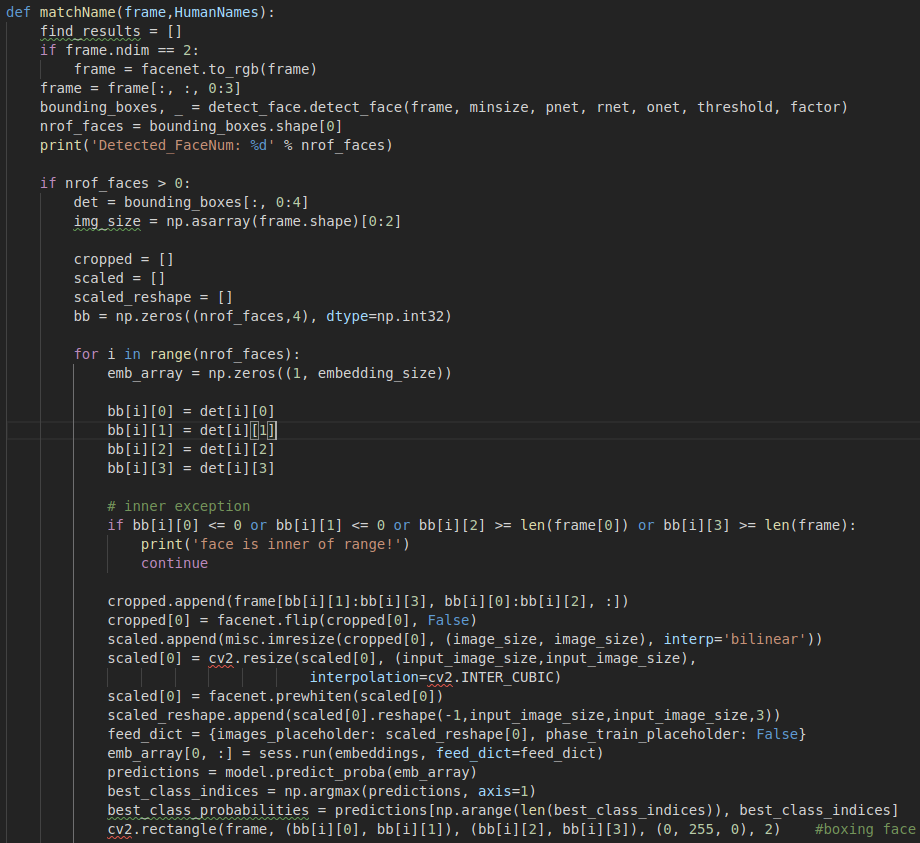
\includegraphics[width=\textwidth]{BoxinFace.png}

The following image is what is produced from the code above. As can be seen, Enrique is recognized with a box that tracks his face. \\ \\

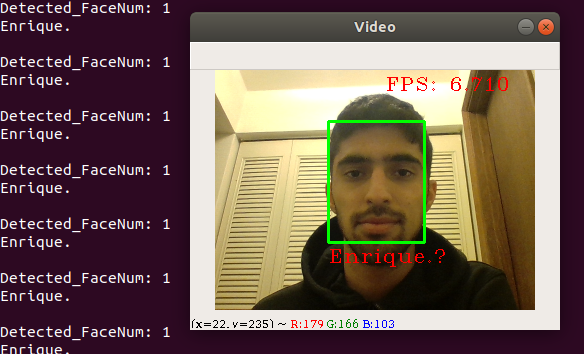
\includegraphics[width=\textwidth]{recognition.png}




\subsection{Utilizing nmap}
The following piece of code utilizes the bash utilities nmap and grep to find all of the devices connected to a router that have a similar IP to the device running the code.
\begin{lstlisting}[language=bash,caption={Utilization of nmap, grep, and regexp}, basicstyle=\scriptsize]
#!/bin/bash
myIP=$( ifconfig | grep -Eo 'inet (addr:)?([0-9]*\.){3}[0-9]*' | grep -Eo '([0-9]*\.){3}[0-9]*' | grep -v '127.0.0.1' )
subNet=$(echo $myIP | grep -Eo '^([0-9]*\.){3}')
nmap -sP $subNet* |  grep -Eo $subNet[0-9]* | grep -v 10.0.0.1$ | grep -v $myIP
\end{lstlisting}

\subsection{HTTP Routing in Python}
The following code handles HTTP requests in python using a library called flask. Note how compact the library makes routing with the use of decorators.
\begin{lstlisting}[language=Python, caption={Server HTTP Routing using flask}, basicstyle=\scriptsize]
import os
import subprocess
from flask import Flask, request, redirect, url_for, send_from_directory

app = Flask(__name__)
app.config['UPLOAD_FOLDER'] = 'assets/'

@app.route('/training-data', methods=['POST'])
def uploadTrainingData():
    file = request.files['file']
    if file: 
        file.save(os.path.join(app.config['UPLOAD_FOLDER'], 'tarPhotos/', file.filename))
        rootDir = os.path.dirname(os.path.realpath(__file__))
        tarCmd = rootDir+'/scripts/decompressPhotos.sh'
        subprocess.call([tarCmd, rootDir, file.filename])
        return file.filename+' upload successful'
    return file.filename+" upload not successful"

@app.route('/classifier', methods=['POST'])
def uploadClassifier():
    file = request.files['file']
    if file: 
        file.save(os.path.join(app.config['UPLOAD_FOLDER'], file.filename))
        return file.filename+'upload successful'
    return file.filename+" upload not successful"

@app.route('/names', methods=['POST'])
def uploadNames():
    file = request.files['file']
    if file: 
        file.save(os.path.join(app.config['UPLOAD_FOLDER'], file.filename))
        return url_for('uploaded_file', filename=file.filename)
    return "file upload not successful"
    
def run():
    app.run(debug=True, port="2000")

if __name__ == '__main__':
	app.run(debug=True)

\end{lstlisting}


\section{Interface Design}
Currently in progress.

\newpage
% ---- Bibliography ----
\begin{thebibliography}{10}
	
	\bibitem{google}
	Fliran Schroff, Dmitry Kalenichenko, James Philbin,
	"FaceNet: A Unified Embedding for Face Recognition and Clusterin",
	\textit{Google Inc.},
	[Online].
	Available: \\\textit{https://arxiv.org/pdf/1503.03832.pdf}.
	[Accessed February 22 2019]
\end{thebibliography}

% --- End Bibliography ----

\end{document}